\subsection{Create Quiz Test} % (fold)
\label{sub:create_quiz_test}
This section contains the test runs performed on the quiz creator.

\clearpage

\subsubsection{Add Question} % (fold)
\label{ssub:add_question}
This ensures that the user is able to succesfully add a question to the current quiz.
\begin{figure}[!htbp]
\centering
\begin{subfigure}{0.5\textwidth}
  \centering
  \includegraphics[width=0.95\linewidth]{testing/create_quiz/add_question/before}
  \caption{Before}
  \label{fig:sub1}
\end{subfigure}%
\begin{subfigure}{0.5\textwidth}
  \centering
  \includegraphics[width=0.95\linewidth]{testing/create_quiz/add_question/after}
  \caption{After}
  \label{fig:sub2}
\end{subfigure}
\caption{Adding a question to the quiz.}
\label{fig:test}
\end{figure}
% subsubsection add_question (end)


\subsubsection{Edit Question} % (fold)
\label{ssub:edit_question}
This ensures that the user is able to succesfully edit a question in the current quiz.
\begin{figure}[!htbp]
\centering
\begin{subfigure}{0.5\textwidth}
  \centering
  \includegraphics[width=0.95\linewidth]{testing/create_quiz/edit_question/before}
  \caption{Before}
  \label{fig:sub1}
\end{subfigure}%
\begin{subfigure}{0.5\textwidth}
  \centering
  \includegraphics[width=0.95\linewidth]{testing/create_quiz/edit_question/after}
  \caption{After}
  \label{fig:sub2}
\end{subfigure}
\caption{Editing a question to the quiz.}
\label{fig:test}
\end{figure}
% subsubsection edit_question (end)


\subsubsection{Delete Question} % (fold)
\label{ssub:delete_question}
This ensures that the user is able to succesfully delete a question in the current quiz.
\begin{figure}[!htbp]
\centering
\begin{subfigure}{0.5\textwidth}
  \centering
  \includegraphics[width=0.95\linewidth]{testing/create_quiz/delete_question/before}
  \caption{Before}
  \label{fig:sub1}
\end{subfigure}%
\begin{subfigure}{0.5\textwidth}
  \centering
  \includegraphics[width=0.95\linewidth]{testing/create_quiz/delete_question/after}
  \caption{After}
  \label{fig:sub2}
\end{subfigure}
\caption{Delete a question in the quiz.}
\label{fig:test}
\end{figure}
% subsubsection delete_question (end)


\subsubsection{Add Category} % (fold)
\label{ssub:add_category}
This ensures that the user is able to succesfully add a custom category to the current quiz.
\begin{figure}[!htbp]
\centering
\begin{subfigure}{0.5\textwidth}
  \centering
  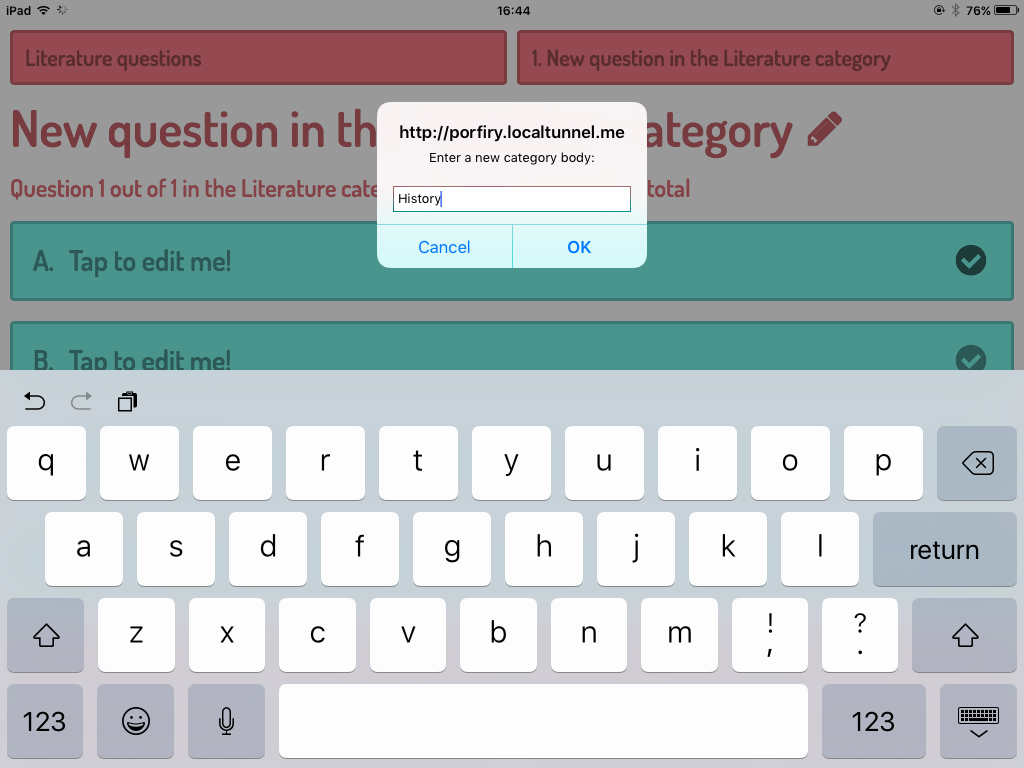
\includegraphics[width=0.95\linewidth]{testing/create_quiz/add_category/during}
  \caption{During}
  \label{fig:sub1}
\end{subfigure}%
\begin{subfigure}{0.5\textwidth}
  \centering
  \includegraphics[width=0.95\linewidth]{testing/create_quiz/add_category/after}
  \caption{After}
  \label{fig:sub2}
\end{subfigure}
\caption{Adding a category to the quiz.}
\label{fig:test}
\end{figure}
As expected, a dialog to enter a category name is shown when the add category button is pressed, and the new category is added successfully. \textit{Success.}
% subsubsection add_category (end)

